\section{Suddivisione del lavoro}
I componenti del gruppo dovranno rivestire ogni ruolo almeno una volta. Possono ricoprire più ruoli contemporaneamente purché non si presentino conflitti di interesse tra i ruoli ricoperti.
	\subsection{Dettaglio Fasi}
		\subsubsection{Analisi}
		Nella fase di Analisi, ciascun componente dovrà ricoprire i seguenti ruoli per il numero di ore indicato nella seguente tabella: \\
		\begin{table}[H]
		\centering
		\begin{tabular}{|c|c|c|c|c|c|c|c|}
			\hline
			\textbf{Nominativo}		& \textbf{PM}	& \textbf{Am}	& \textbf{An}	& \textbf{Pt}	& \textbf{Pr}	& \textbf{Ve}	& \textbf{Ore totali}     \\
			\hline
			Salvatore Pilò			& 10	& 		& 12	&		&		&		& 22 \\
			Fabio Massignan			&		& 5		&		&		&		& 16	& 21 \\
			Sebastiano Bertolin		&		& 4		& 15	&		&		&		& 19 \\
			Davide Santimaria		&		& 4		& 16	&		&		&		& 20 \\
			Malick Bodian			& 9		&		&		&		&		& 13	& 22 \\
			Gianmarco Salmistraro	&		& 4		& 15	&		&		& 2		& 21 \\
			\hline
		\end{tabular}
		\end{table}
		I valori sono riassunti nel seguente grafico, che rappresenta in maniera visiva per quante ore un membro abbia ricoperto un determinato ruolo. \\
		\begin{figure}[H]
			\centering
			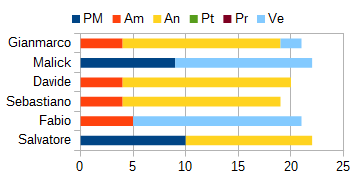
\includegraphics[scale=1]{immagini/grafici/analisi-barra.png}
			\caption{Ore per componente, fase di Analisi}
		\end{figure}
		\subsubsection{Analisi di Dettaglio}
		Nella fase di Analisi di Dettaglio, ciascun componente dovrà ricoprire i seguenti ruoli per il numero di ore indicato nella seguente tabella: \\
		\begin{table}[H]
		\centering
		\begin{tabular}{|c|c|c|c|c|c|c|c|}
			\hline
			\textbf{Nominativo}		& \textbf{PM}	& \textbf{Am}	& \textbf{An}	& \textbf{Pt}	& \textbf{Pr}	& \textbf{Ve}	& \textbf{Ore totali}     \\
			\hline
			Salvatore Pilò			&		& 		& 4		&		&		& 2		& 6 \\
			Fabio Massignan			& 1		& 		& 4		&		&		& 		& 5 \\
			Sebastiano Bertolin		&		& 		& 5		&		&		&		& 5 \\
			Davide Santimaria		&		& 2		&		&		&		& 3		& 5 \\
			Malick Bodian			& 		& 		& 4		&		&		& 		& 4 \\
			Gianmarco Salmistraro	&		& 		& 5		&		&		& 		& 5 \\
			\hline
		\end{tabular}
		\end{table}
		I valori sono riassunti nel seguente grafico, che rappresenta in maniera visiva per quante ore un membro abbia ricoperto un determinato ruolo. \\
		\begin{figure}[H]
			\centering
			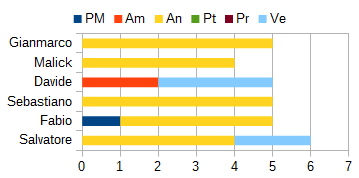
\includegraphics[scale=1]{immagini/grafici/analisi_dettaglio-barra.png}
			\caption{Ore per componente, fase di Analisi di Dettaglio}
		\end{figure}
		\subsubsection{Progettazione Architetturale}
		Nella fase di Progettazione Architetturale, ciascun componente dovrà ricoprire i seguenti ruoli per il numero di ore indicato nella seguente tabella: \\
		\begin{table}[H]
		\centering
		\begin{tabular}{|c|c|c|c|c|c|c|c|}
			\hline
			\textbf{Nominativo}		& \textbf{PM}	& \textbf{Am}	& \textbf{An}	& \textbf{Pt}	& \textbf{Pr}	& \textbf{Ve}	& \textbf{Ore totali}     \\
			\hline
			Salvatore Pilò			& 		& 5 	& 2		& 22	&		&		& 29 \\
			Fabio Massignan			&		& 		& 2		& 10	&		& 15	& 27 \\
			Sebastiano Bertolin		& 5		& 		& 4		& 16	&		&		& 25 \\
			Davide Santimaria		&		& 		& 6		&		&		& 20	& 26 \\
			Malick Bodian			& 		& 2		& 5		& 21	&		& 		& 28 \\
			Gianmarco Salmistraro	& 5		& 		& 2		& 20	&		& 		& 27 \\
			\hline
		\end{tabular}
		\end{table}
		I valori sono riassunti nel seguente grafico, che rappresenta in maniera visiva per quante ore un membro abbia ricoperto un determinato ruolo. \\
		\begin{figure}[H]
			\centering
			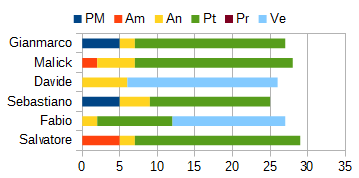
\includegraphics[scale=1]{immagini/grafici/progettazione_architetturale-barra.png}
			\caption{Ore per componente, fase di Progettazione Architetturale}
		\end{figure}
		\subsubsection{Progettazione di Dettaglio e Codifica}
		Nella fase di Progettazione di Dettaglio e Codifica, ciascun componente dovrà ricoprire i seguenti ruoli per il numero di ore indicato nella seguente tabella: \\
		\begin{table}[H]
		\centering
		\begin{tabular}{|c|c|c|c|c|c|c|c|}
			\hline
			\textbf{Nominativo}		& \textbf{PM}	& \textbf{Am}	& \textbf{An}	& \textbf{Pt}	& \textbf{Pr}	& \textbf{Ve}	& \textbf{Ore totali}     \\
			\hline
			Salvatore Pilò			& 		& 		& 2		& 20	&		& 30	& 52 \\
			Fabio Massignan			& 5		& 		&		& 15	& 30	& 		& 50 \\
			Sebastiano Bertolin		&		& 		& 		& 16	& 18	& 16	& 50 \\
			Davide Santimaria		& 5		& 		& 		& 16	& 28	&		& 49 \\
			Malick Bodian			& 		& 6		&		& 16	&		& 28	& 50 \\
			Gianmarco Salmistraro	&		& 		& 		& 20	& 30	& 10	& 50 \\
			\hline
		\end{tabular}
		\end{table}
		I valori sono riassunti nel seguente grafico, che rappresenta in maniera visiva per quante ore un membro abbia ricoperto un determinato ruolo. \\
		\begin{figure}[H]
			\centering
			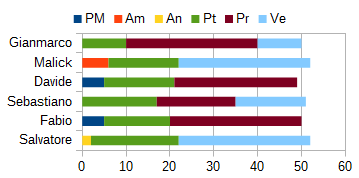
\includegraphics[scale=1]{immagini/grafici/progettazione_dettaglio_codifica-barra.png}
			\caption{Ore per componente, fase di Progettazione di Dettaglio e Codifica}
		\end{figure}
		\subsubsection{Verifica e Validazione}
		Nella fase di Verifica e Validazione, ciascun componente dovrà ricoprire i seguenti ruoli per il numero di ore indicato nella seguente tabella: \\
		\begin{table}[H]
		\centering
		\begin{tabular}{|c|c|c|c|c|c|c|c|}
			\hline
			\textbf{Nominativo}		& \textbf{PM}	& \textbf{Am}	& \textbf{An}	& \textbf{Pt}	& \textbf{Pr}	& \textbf{Ve}	& \textbf{Ore totali}     \\
			\hline
			Salvatore Pilò			& 9		& 		& 		&		& 10	&		& 19 \\
			Fabio Massignan			&		& 2		&		& 8		&		& 14	& 24 \\
			Sebastiano Bertolin		&		& 2		& 		& 4		&		& 19	& 25 \\
			Davide Santimaria		&		& 2		& 		& 3		&		& 19	& 24 \\
			Malick Bodian			& 2		& 7		&		&		& 11	& 		& 20 \\
			Gianmarco Salmistraro	&		& 9		& 		&		& 12	& 2		& 23 \\
			\hline
		\end{tabular}
		\end{table}
		I valori sono riassunti nel seguente grafico, che rappresenta in maniera visiva per quante ore un membro abbia ricoperto un determinato ruolo. \\
		\begin{figure}[H]
			\centering
			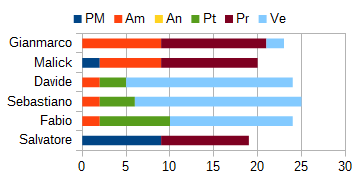
\includegraphics[scale=1]{immagini/grafici/validazione-barra.png}
			\caption{Ore per componente, fase di Verifica e Validazione}
		\end{figure}
	\subsection{Totali}
		\subsubsection{Ore totali con investimento}
		Le ore totali, comprese quelle di investimento, dedicate da ciascun componente all'intero progetto saranno le seguenti: \\
		\begin{table}[H]
		\centering
		\begin{tabular}{|c|c|c|c|c|c|c|c|}
			\hline
			\textbf{Nominativo}		& \textbf{PM}	& \textbf{Am}	& \textbf{An}	& \textbf{Pt}	& \textbf{Pr}	& \textbf{Ve}	& \textbf{Ore totali}     \\
			\hline
			Salvatore Pilò			& 19	& 5		& 20	& 42	& 10	& 32	& 128 \\
			Fabio Massignan			& 6		& 7		& 6		& 33	& 30	& 45	& 127 \\
			Sebastiano Bertolin		& 5		& 6		& 24	& 36	& 18	& 35	& 124 \\
			Davide Santimaria		& 5		& 8		& 22	& 19	& 28	& 42	& 124 \\
			Malick Bodian			& 11	& 15	& 9		& 37	& 11	& 41	& 124 \\
			Gianmarco Salmistraro	& 5		& 13	& 22	& 30	& 42	& 14	& 126 \\
			\hline
		\end{tabular}
		\end{table}
		I valori sono riassunti nel seguente grafico, che rappresenta in maniera visiva per quante ore un membro abbia ricoperto un determinato ruolo. \\
		\begin{figure}[H]
			\centering
			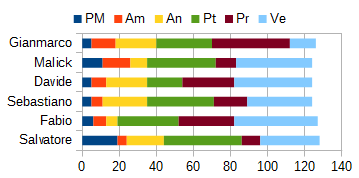
\includegraphics[scale=1]{immagini/grafici/riepilogo_conclusivo-barra.png}
			\caption{Ore per componente totali con investimento}
		\end{figure}
		\subsubsection{Ore rendicontate}
		Le ore totali rendicontate dedicate da ciascun componente all'intero progetto saranno le seguenti: \\
		\begin{table}[H]
		\centering
		\begin{tabular}{|c|c|c|c|c|c|c|c|}
			\hline
			\textbf{Nominativo}		& \textbf{PM}	& \textbf{Am}	& \textbf{An}	& \textbf{Pt}	& \textbf{Pr}	& \textbf{Ve}	& \textbf{Ore totali}     \\
			\hline
			Salvatore Pilò			& 9		& 5		& 4		& 42	& 10	& 30	& 100 \\
			Fabio Massignan			& 5		& 2		& 2		& 33	& 30	& 29	& 101 \\
			Sebastiano Bertolin		& 5		& 2		& 4		& 36	& 18	& 35	& 100 \\
			Davide Santimaria		& 5		& 2		& 6		& 19	& 28	& 39	& 99 \\
			Malick Bodian			& 2		& 15	& 5		& 37	& 11	& 28	& 98 \\
			Gianmarco Salmistraro	& 5		& 9		& 2		& 30	& 42	& 12	& 100 \\
			\hline
		\end{tabular}
		\end{table}
		I valori sono riassunti nel seguente grafico, che rappresenta in maniera visiva per quante ore un membro abbia ricoperto un determinato ruolo. \\
		\begin{figure}[H]
			\centering
			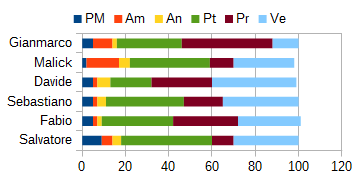
\includegraphics[scale=1]{immagini/grafici/orario_rendicontato-barra.png}
			\caption{Ore per componente totali rendicontate}
		\end{figure}